\documentstyle[fancyfig,psy,iot92,psfig]{article}
\psfigurepath{../postscript/}
%\psdraft
\newcommand{\x}[2]{\mbox{$#1\times#2$}}


\showwherepublished
\firstpage{22}

%% Remember \seriation and \APAitemize

\begin{document}
\bibliographystyle{psy}


\author{Richard Dallaway}
\title{Connectionism: Animal Models for\\Cognitive Science?}
\email{richardd@cogs.susx.ac.uk}
\maketitle

%\begin{quote}{\changefont{helvetica}\bf ABSTRACT}\hspace{3mm}%
%
\begin{abstract}
Connectionism is to the mind as guinea pigs are to the skin.
Guinea pigs, when shaved, show similar skin reactions to those observed of
humans.
Likewise, certain connectionist systems (e.g., three-layer
networks trained with backpropagation) show similar behaviours to those
noted of human minds.  However, although these ``animal models'' inform
theories, in themselves they
explain little. The implication is that we should treat
connectionist networks as objects of study, rather than as theories of the
mind, or even simulations of theories. This suggestion, by
\citeA{mcclnetw}, concludes that there is a difference between classical
cognitivism and connectionism when it comes to the relationship between
models and theories.
%\end{quote}
\end{abstract}
\section*{Introduction}

Connectionist networks have many properties that suggest that they are good
tools for modelling some aspects of cognition \cite{micro}. However, a
recent paper by \citeA{mcclnetw} highlights the fact that the relationship
between connectionist models and theories of cognition is far from simple.
This paper is a short review of McCloskey's suggestions, illustrated with
examples from my own work.  What follows consists mostly of statements of
how connectionism works today, rather than in principle arguments of what
is or is not possible.  It is also limited to the implications of using a
particular kind of architecture (trained, layered networks), and focusses on
cognitive (as opposed to neural) models.

\paragraph{Memory for multiplication}  The example connectionist model used
in the following discussion is one for modelling adult memory for
multiplication facts.
There are some well established results on memory for
multiplication \cite{camp85},
the most striking of which are stated here.
When reaction time is measured, it turns out that subjects can
answer small problems (such as $\x34=12$) faster than large problems
($\x89=72$). There are exceptions to this rule, most notably the five
times table and ``tie'' problems (e.g., \x22
and \x33). The mistakes made when
recalling multiplication facts also follows a pattern.  Any wrong answer
given to, say, \x34 will probably be in the three or four times table.

A connectionist network has been built to capture these phenomena
\cite{dallmemo}.  Apart from modifications to measure reaction time, the
network conforms to the stereotypical connectionist architecture: an input
encoding (of digits to be multiplied) is connected to a layer of hidden
units which feed to a set of output units (representing products).  The
whole system is trained with backpropagation.

Given that the model does captures some of the behaviour observed of adults
(and whether it does or does is of little importance here), the
question to be addressed is: how well does the model {\em explain} human
behaviour?

\section*{Theory and simulation}

A running simulation is usually taken to be proof of an explicit
theory.  That is, in classical cognitivism, you cannot write a program
unless you have all the details specified in the theory. The behaviour of
the running program can then suggest new directions for the theory, be used
for predictions, and help confirm or refute aspects of the theory
\cite{newecomp}.

This is not the way connectionism works. Vague intuitions about the domain
can be implemented (in terms of an input to output mapping), and any
underdeveloped ideas or unspecified details are filled in by the learning
algorithm. On the surface this sounds like a useful way of working, but the
usual result is a complex black-box system that we don't yet know how to
analyse.  As McCloskey notes: ``In a sense the modeler `grows' the network
rather than building it.  And, just as a gardener's ability to grow a plant
from a seed does not imply that the gardener has an explicit theory of
plant physiology, the ability to grow a network that mimics in some
respects a human cognitive function does not demonstrate that the modeler
has an explicit theory of that function'' \citeyear[p.~391]{mcclnetw}.


\paragraph{What is a theory, anyway?}  McCloskey argues that this is no way
to conduct research.  The starting point of a theory should be at a level
more abstract that that of a single simulation, identifying how a cognitive
function is carried out and how this functioning leads to the observed
behaviour.  In the context of connectionism it's not yet apparent what
language should be used---but presumably it is not the same language used
for symbolic systems \cite{ptc}. In the case of mental arithmetic, we want
the theory to tell us which factors determine the response time for, say,
problems involving a five, and which are irrelevant.  When the simulation
successfully models some aspect of behaviour, we'd like to know which
aspects of the theory can be credited; or conversely, when the simulation
fails, which assumptions are to blame, and whether or not the failure is a
significant.


\paragraph{We don't understand networks (yet)} Current
connectionism methodology
fails as a theory (as described above) because we do
not yet have the tools for understanding networks or the training
procedures used to create these networks \cite{minsperc}.  If we did
understand these systems, the training of networks would have the same
status as the writing of symbolic programs:  an exercise to ensure the
theory is explicit (which should not produce too many surprises).

This gap in our understanding is due to the
poverty of the techniques available to study networks. When trying to
understand how a network solves some problem, connectionists often resort
to a set of visualization tools \cite{hanswhat}, such as cluster
analysis, principle components analysis, and Hinton diagrams.  The idea
here is to find answers to questions like: What knowledge does the system
encode? How is that knowledge used? and (less often) How did that knowledge
get there?  These are hard questions that are not fully answered by current
analysis techniques.

One approach which I took towards analysing the multiplication network
mentioned above, was to look at how each hidden unit reacted to each
multiplication problem. Although it was superficially interesting to see
that certain units reacted to groups of problems (such as ``small''
products, or ``sevens''), the exercise has not shed much light on why
those weights develop, or which aspects of the simulation most
influence their development.

We can hope that techniques will be developed to enable us to fully
understand the functioning of networks. The replies to
\citeauthor{hanswhat}'s article range from the optimistic to positively
pessimistic on this point: ``\ldots actual large nets produced in the
future will be {\em computationally irreducible}, in that no analysis in
terms smaller than the nets themselves will give anything like a really
detailed and accurate account of how they work'' \cite[p.~508]{suppprob}.
Without a way to understand how a change in the input representation (for
example) would change the results of a (non-trivial) simulation, there is
no way to assign credit or blame to aspects of the simulation. Note that
this implies that even if a connectionist modeller is working from a
detailed theory, there is  no obvious way to show that the network does
implement the theory.


Of course, no-one would want to argue that a single connectionist network
constitutes a theory of some phenomena. A theory should specify important
features of the domain (such as the input
representation), and a number of simulations
could help confirm of disclaim the importance of such features.  In
addition, multiple simulations could quantify the importance of other
features (like the number of hidden units) which are not usually specified
in a theory. For any interesting problem, though, there will be too many
parameters to test exhaustively.



\section*{The need for better analysis}

This lack of understanding shows itself when evaluating various claims that
are made for connectionist models. For example, there is some support for a
``dual process'' theory in models of memory for multiplication facts
\cite{mcclfact}.  It is assumed that some kinds of spreading activation is
used to recall most facts, but that a rule is used for multiplying by zero
($\x0N=0$).  Evidence for this comes from the kinds of mistakes subjects
make for zero problems (they are mostly of the form $\x0N=N$). However, if
the connectionist network for multiplication (mentioned above) was fully
consistent with these findings it would be tempting to say that there is no
need for a dual mechanism, and that a single mechanism (the network) can
accommodate the findings.  (In fact the network isn't consistent with the
findings; but see \citeA{dallspee} for the full story.)

To say that a number of tasks can be achieved with a single mechanism is
trivially true: you could just as well say that all of vision, language and
reasoning are performed with a single mechanism (the brain).  However, such
claims are interesting if they are true ``\ldots at levels relevant for
cognitive theorizing'', which means ``\ldots at levels appropriate for
stating generalizations\ldots'' about the domain \cite[p.~391]{mcclnetw}.
At the moment we don't have the tools to understand networks at this level,
and as such cannot evaluate these kinds of theoretical claims.

Finally, note how the connectionist model of arithmetic memory compares to
the symbolic account (for
addition) shown in figure~\ref{min}. This model is
easy to analyse: it's obvious what determines response time (the
magnitude of the smaller number).

\begin{fancyfigure}\smallskip
\centerline{\psfig{file=minmodel.ps,width=11cm}}
\caption{The MIN model of cognitive counting, where is subject is assumed
to be unconsciously incrementing a counter when performing mental
addition.  When calculating $a+b$, a counter is set equal to the larger
number, and then the counter is repeatedly incremented
(see review in \protect\citeay{resndeve}).}
\label{min}
\end{fancyfigure}


\section*{Animal models}

As already mentioned, connectionism has many interesting notions: learning
internal representations, self-organization, emergent properties, and so
on. It seems that for some researchers the attraction of these properties,
coupled with the perceived inadequacies of symbolic simulations
seems to outweigh the added cost of analysis.
However, as described above, a connectionist model does not qualify as a
simulation of a theory.
If this
is the case, perhaps we should stop viewing connectionism as a model, and
start considering other roles it might play.

Animal models are things like guinea pigs. The skin of a guinea pig is a
good model of human skin to the degree in which it shows the same kinds of
allergic reactions that human skin shows \cite{bothwhy}. It is supposed
that the animal shares some ``critical features'' with the equivalent human
system, and that the animal system will be in some sense simpler, and hence
more amenable to analysis.  In addition, it is possible to perform
experiments on animals that cannot be performed on human subjects.  On the
other hand, it may turn out that the similarity between the human and
animal system is superficial, and that there are no shared features of
interest. (See also \citeauthor{hendcuri}, this volume, for more problems
with studying animal systems.)

The guinea pig is not a theory of human skin allergy, nor even a simulation
of a theory:  it is an object of study.  Knowledge about such an object is
not expected to contribute directly to the understanding of the human
system.  Instead, the object contributes to the development
of a theory of the corresponding human system.

McCloskey suggests that connectionist networks should be treated as a kind
of animal model for cognitive science. (To clarify: the analogy with animal
models is {\em not\/} alluding to any biological similarity or
plausibility.) The hope is that the ability of a network to replicate some
phenomena is due to some ``critical features'' shared with humans. ``If by
studying the network we can gain some understanding of it structure and
functioning at a level relevant for cognitive theorizing, this
understanding might aid in developing a theory of human cognitive
processes'' \cite[p.~393]{mcclnetw}.  Connectionism has all the advantages
of animal models, with the added bonuses that come from computer
simulations (e.g., knowing all the details about the simulations, being
able to stop and restart the simulation from any point, etc). Connectionism
also shares some of the disadvantages: despite similar behaviour, there may
be no interesting common features between networks and humans.

Working within the animal model analogy means turning away from the usual
iterative ``theory-model'' cycle (where a model built from a theory may
suggest changes to the theory, which leads to a new model\ldots).  Instead,
observations of the model suggest changes to the theory, but you cannot
(currently) associate aspects of the model to features in the theory (as
discussed above).


\section*{Conclusions}

McCloskey's analogy to animal models suggests that two, interrelated
directions must be explored.  First, although demonstrating that networks
can mimic human behaviour is important, better analysis tools need to be
developed.  Second, a language is needed for stating connectionist theories
of
cognition.   Presumably, the notions employed by the analysis tools will
play a major role in the language in which connectionist theories are to be
stated. This assumes that the analysis will provide insights that are
independent from any particular network, and are at a level ``relevant for
cognitive theorizing.''

% One possibility is that notions from the study of dynamic systems
% \cite{vangptc} will filter back up to change connectionism
% in much the same way as subsymbolic research has changed various notions,
% like ``symbol''.  van~Gelder identifies himself as a ``dynamicists'', and
% makes a number of claims, including: ``The most appropriate tools for the
% study of cognition are dynamical modelling and dynamical systems theory''
% \citeyear[p.~643]{vangptc}.  He also notes that symbolic and connectionist
% systems are dynamic systems, but ``\ldots only a relatively small portion
% of connectionist researchers bring genuinely dynamical methods to bear in
% their descriptions of network functioning or cognitive processes\ldots''
% (p.~642).

McCloskey's analogy to animal models serves as a useful interim measure
until new analysis methods become available, or a understanding of parallel
computation is gained. The analogy suggests that a viable research strategy
is to identify the set of connectionist properties (combinations of
architectures and representations) which seem to share features with a
human system. One way to do this is to first compare a number of
connectionist networks with a view to identifying the generally important
features (rather than the ones that are specific to a particular
simulation); and then  use this distilled set of features to aid the
development of a theory of the domain.  For example, there are three
published connectionist models of memory for multiplication: one based on
the brain-state-in-a-box algorithm \cite{andestud}; another using
mean-field theory \cite{mcclmath}; and one based on backpropagation
\cite{dallmemo}. All three use different ways to measure response time,
different input and output representations, training sets, numbers of
hidden units, and so on, yet all show some degree of match to human
behaviour.  If connectionism has any claim on sharing critical mechanisms
(in this case, memory) with human systems, some of the features exploited
by these models should be independent of the particular details of any one of
the systems, and should contribute to a theory of mental arithmetic.

\bibliography{bib}
\end{document}
